\section{Anden iteration}

\subsection{Transformator}
Figur~\ref{fig: Primarinduktans} viser induktansen målt i transformatorens primærvikling, ved et frekvenssweep $100Hz$ til $1MHz$.. 
\begin{figure}[H]
	\center
	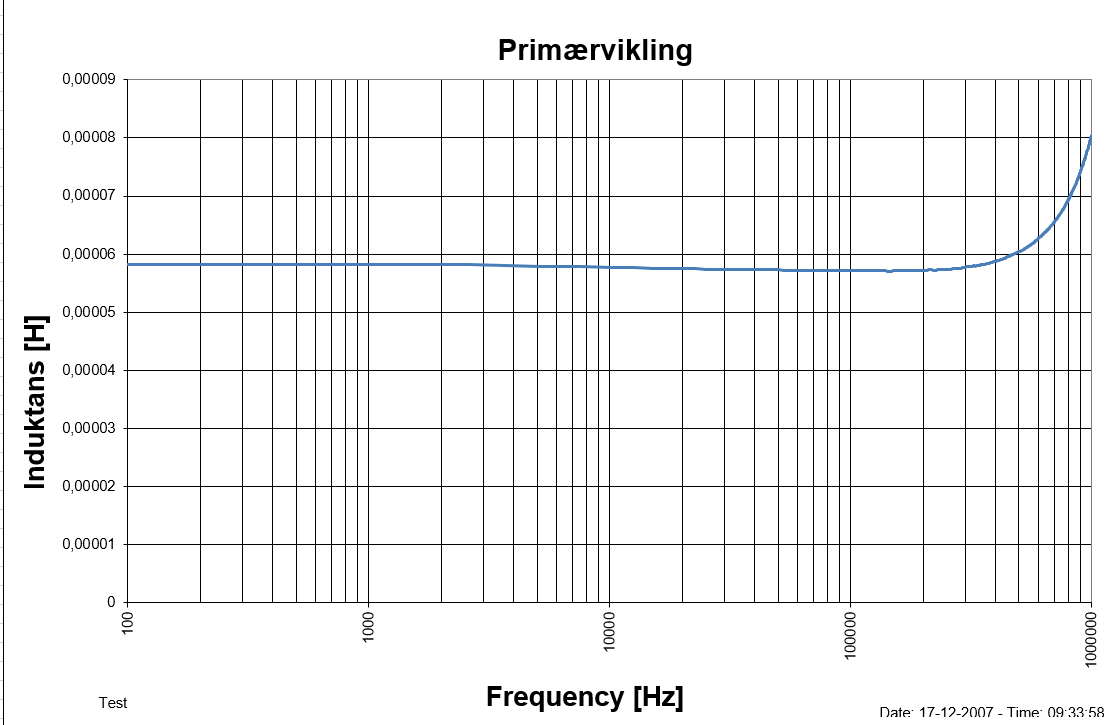
\includegraphics[max width=0.7\linewidth]{../dokumentation/tex/2iteration/billeder/Primarinduktans.png}
	\caption{Målt induktans i primær vikling}
	\label{fig: Primarinduktans}
\end{figure}
Ud fra de præcise værdier, som er vedlagt i bilagsmappen, findes induktansen ved 100kHz til $57.7\micro H$

Figur~\ref{fig: leakageinductance} viser spredningsselvinduktansen målt i transformatoren, ved et frekvenssweep på $100Hz$ til $1MHz$.
\begin{figure}[H]
	\center
	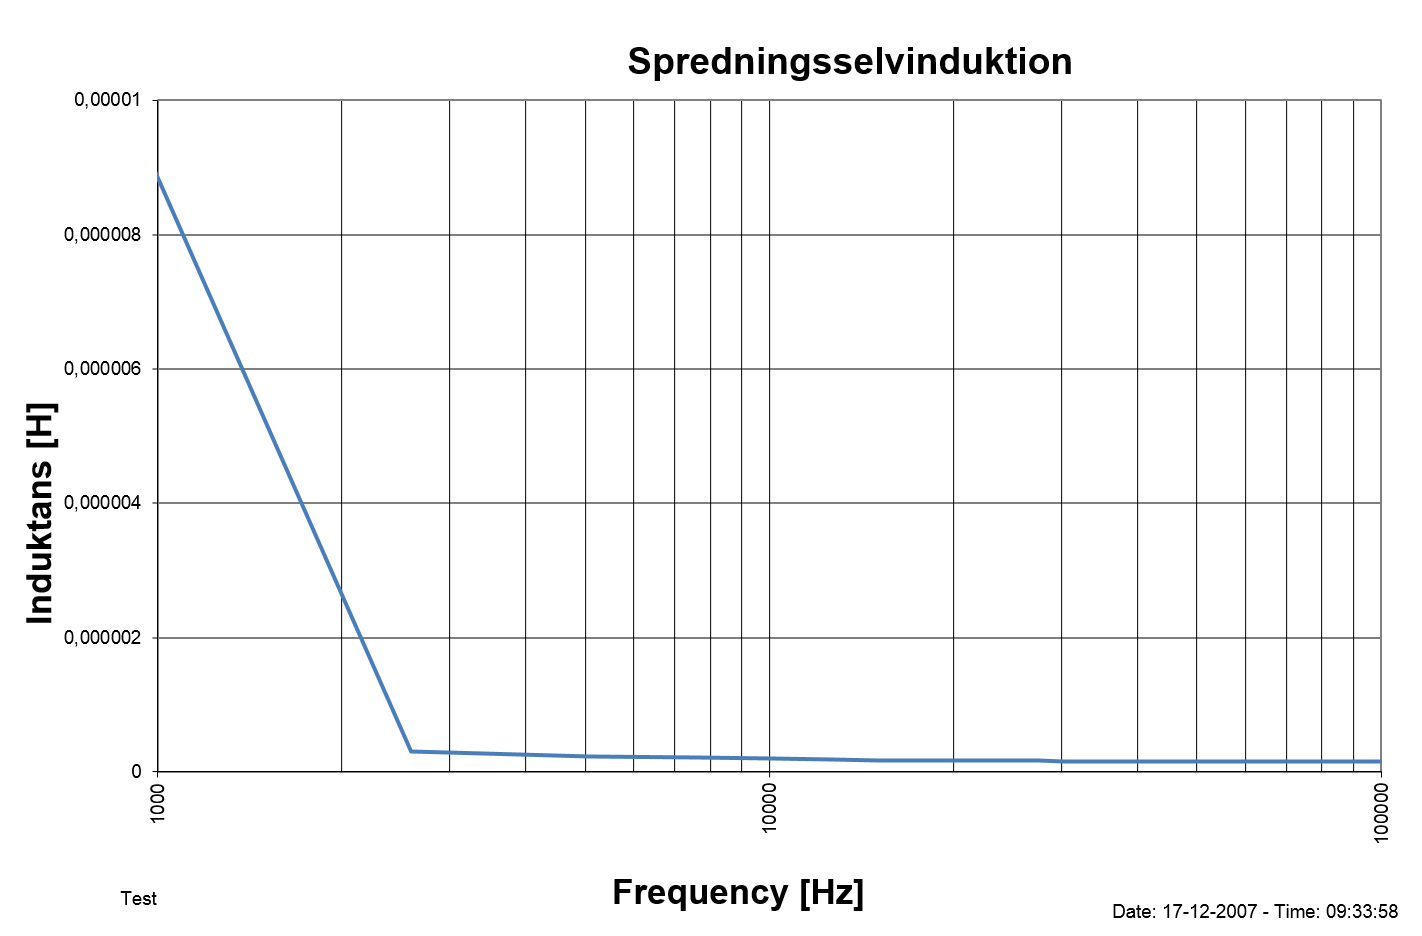
\includegraphics[max width=0.7\linewidth]{../dokumentation/tex/2iteration/billeder/Spredningsselvinduktion.png}
	\caption{Målt spredningsselvinduktion i transformator}
	\label{fig: leakageinductance}
\end{figure}

\subsection{Integrationtest - Constant load}

\subsubsection{Udgang}
Figur~\ref{fig: Out26V} viser det realiserede spændingsoutput ved 26V. Kanal et viser spændingsoutputtet, mens kanal to viser gate spændingen for MOSFET'en. Kanal to er brugt til at trigge på, ved alle constant load målingerne. 
\begin{figure}[H]
	\center
	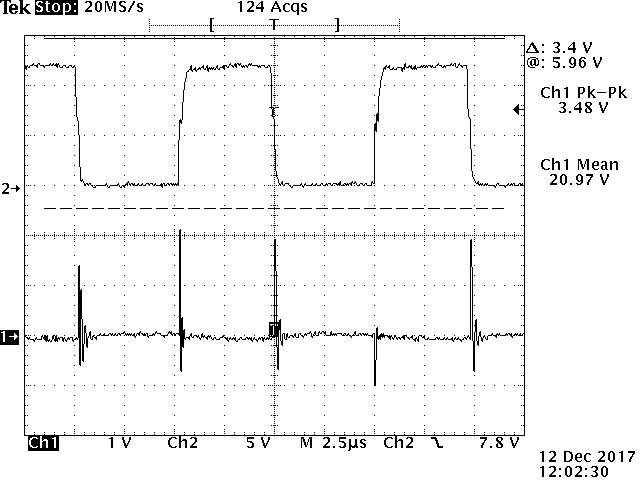
\includegraphics[max width=0.7\linewidth]{../dokumentation/tex/2iteration/billeder/Realisering/udgang_f_filter_2iteration.png}
	\caption{Spændingsoutput ved 26V}
	\label{fig: Out26V}
\end{figure}
Spændingen aflæses til at ligge på 20.97V. Yderligere observeres det, at der er swithing spikes på omkring 3.48V pk-pk.

\subsubsection{MOSFET og diode}
Figur~\ref{fig: privolt} viser drain spændingen for MOSFET'en på kanal et, som også svarer til spændingen over den primære vikling i transformatoren.
\begin{figure}[H]
	\center
	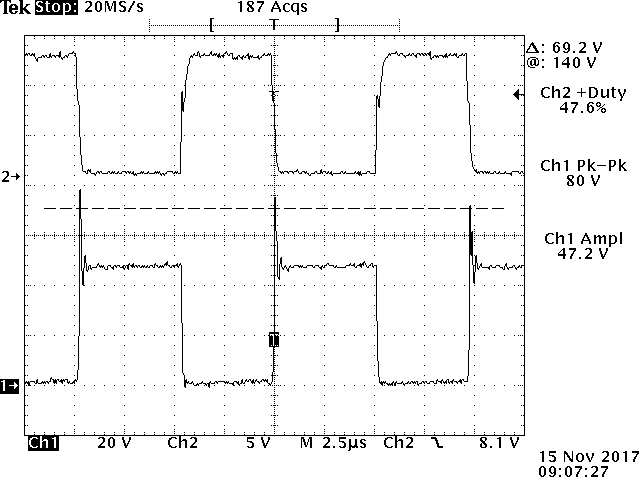
\includegraphics[max width=0.7\linewidth]{../dokumentation/tex/2iteration/billeder/Realisering/Transformator_Primar.png}
	\caption{Primær spænding}
	\label{fig: privolt}
\end{figure}
Spændingen over den primære vikling aflæses til en peak på 80V. Derudover aflæses den stationære spænding at ligge på 47V. 
På figur~\ref{fig: prizoom} er der zoomet ind på svingningerne omkring peakspændingen, som observeres ovenfor.
\begin{figure}[H]
	\center
	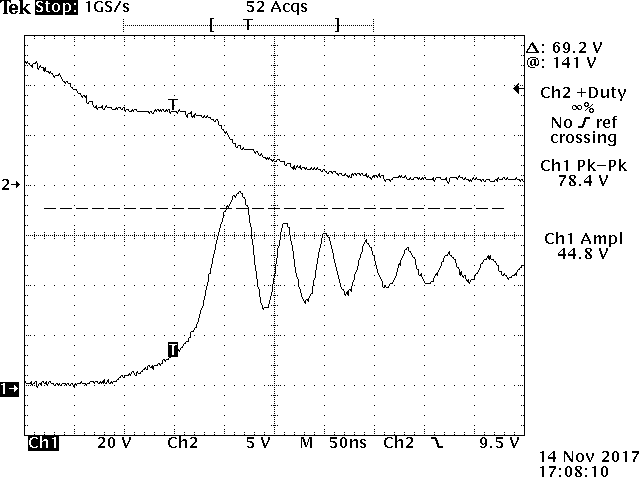
\includegraphics[max width=0.7\linewidth]{../dokumentation/tex/2iteration/billeder/Realisering/Transformator_Primarzoom.png}
	\caption{Zoomet på primær peak}
	\label{fig: prizoom}
\end{figure}
Svingningen for en periode aflæses til 40ns. Det svarer til en frekvens på $25MHz$

På figur~\ref{fig:sek} ses spændingen på anoden af dioden på kanal et, som også svarer til spændingen over den sekundære vikling.
\begin{figure}[H]
	\center
	\includegraphics[max width=0.7\linewidth]{../dokumentation/tex/2iteration/billeder/Realisering/Transformator_sekundar.png}
	\caption{Sekundær spænding}
	\label{fig:sek}
\end{figure}
Spændingen over den sekundære vikling aflæses til at have en peakspænding på ca. 60V. Herudover en stationær spænding på ca. 45V. 
På figur~\ref{fig:sekzoom} zoomes der igen ind på svingningerne der opstår efter peaken.
\begin{figure}[H]
	\center
	\includegraphics[max width=0.7\linewidth]{../dokumentation/tex/2iteration/billeder/Realisering/Transformator_sekundarzoomrise.png}
	\caption{Zoomet på sekundær peak}
	\label{fig:sekzoom}
\end{figure}
Svingningen for en periode aflæses til 35ns, hvilket svarer til en frekvens på $28.57MHz$

I tabel~\ref{tab:MOSDIODE} ses sammenhængen mellem simulering og realisering for dioden og MOSFET'en.
\begin{table}[H] 			
	\centering
	\begin{tabularx}{\textwidth}{|X|l|l|l|l|}
		\hline
		& \multicolumn{2}{|X|}{\textbf{Simulering}} & \multicolumn{2}{|X|}{\textbf{Realisering}} \\ \hline
		& MOSFET & Diode & MOSFET & Diode \\ \hline
		Stationær spænding & $48V$ & $46V$ & $47V$ & $45V$ \\ \hline
		Peakspænding & $93V$ & $80V$ & $80V$ & $60V$ \\ \hline
		Svingningsfrekvens & $29.41M\hertz$ & $33.33M\hertz$ & $25.00M\hertz$ & $28.57M\hertz$ \\ \hline
	\end{tabularx}
	\caption{Simulering og realisering af spændinger over MOSFET og diode}
	\label{tab:MOSDIODE}
\end{table}

\subsubsection{PWM-controller}
Tabel~\ref{tab:resultat_PWM} viser analyse-, simulering- og realiseringsresultaterne for de centrale dele af PWM-controlleren. Det indebærer switch-frekvens($f_s$), switch-tid($T_{ch})$ og stigetiden på filtret til current-sense kredsløbet($T_r$)
\begin{table}[H] 			
	\centering
	\begin{tabularx}{\textwidth}{|X|c|c|c|}
		\hline
		\textbf{Frekvens} & \multicolumn{3}{|c|}{\textbf{Resultat}} 		\\ \hline
		& A & S & R 									\\ \hline 
		$f_s$ & $100k\hertz$ & $99.01k\hertz$ & $95.8k\hertz$ 									\\ \hline
		$T_{ch}$ & $138.7ns$ & $103ns$ & $120ns$ 									\\ \hline
		$T_r$ & $300ns$ & $280ns$ & $350ns$ 									\\ \hline
	\end{tabularx}
	\caption{Resultater for analyse, simulering og realisering af udvalgte dele af PWM-controlleren}
	\label{tab:resultat_PWM}
\end{table}

\subsection{Tab}
Tabel~\ref{tab:realisering_tab} giver et overblik over sammenhængen i mellem det analyserede, simulerede og realiserede tab.
\begin{table}[H] 			
	\centering
	\begin{tabularx}{\textwidth}{|X|l|l|l|}
		\hline
		\textbf{\large Komponent} & \multicolumn{3}{|l|}{\textbf{\large Tab}} \\ \hline
		& A & S	& R\\ \hline
		\textbf{Transformator samlet} & $1.46\watt$ & $1.62\watt$ & $0.8\watt$\\ \hline 
		Kernetab & $366m\watt$ & $311m\watt$ &  \\ \hline
		Kobbertab & $1.09\watt$ & $1.31\watt$ & \\ \hline
		& &	& \\ \hline
		\textbf{MOSFET samlet} & $5.55\watt$ & $4.45\watt$ & $5.03\watt$\\ \hline
		Conductiontab & $1.06\watt$ & & \\ \hline
		Switchtab & $4.49\watt$ &  &    \\ \hline
		& &	& \\ \hline
		\textbf{Diode} & $1.13\watt$ & $1.47\watt$ & $1.77\watt$\\ \hline
		& &	& \\ \hline
		\textbf{CS modstands tab} & $1.52\watt$ & $2.03\watt$ & \\ \hline
		& &	& \\ \hline
		\textbf{Total tab} & $9.67\watt$ & $9.57\watt$ & $8.6\watt$\\ \hline
	\end{tabularx}
	\caption{Oversigt over analyseret, simuleret og realiseret tab}
	\label{tab:realisering_tab}
\end{table}

\subsection{Integrationstest - Gain-fase måling}

Figur~\ref{fig:realisering_gain_fase_power} viser det realiserede bode plot for powermodulet sammen med det analyserede.
\begin{figure}[H]
	\center
	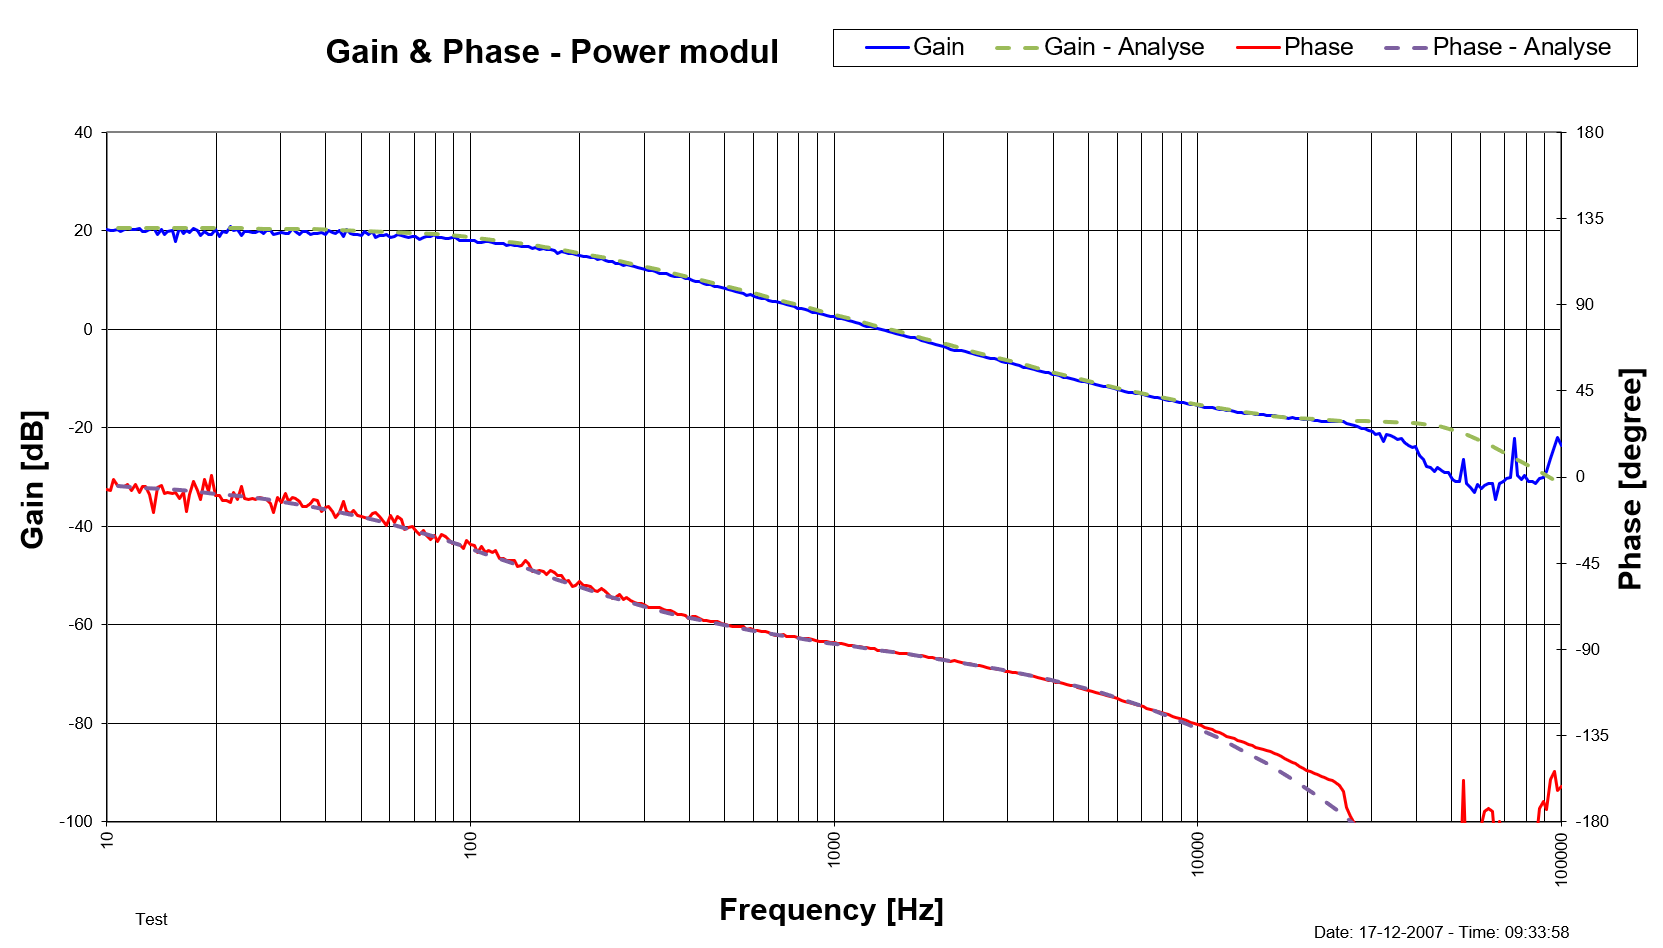
\includegraphics[max width=0.7\linewidth]{../dokumentation/tex/2iteration/billeder/Realisering/Realisering_gain_fase_power.png}
	\caption{Realiseret og analytisk gain-fase for power modul}
	\label{fig:realisering_gain_fase_power}
\end{figure}
Den blå linje er fasen for det realiserede, mens gain er den røde linje. Den grønne stiplede linje stammer fra den analyserede fase og den lila stiplede er det analyserede gain. Båndbredden aflæses for begge dele til $1400Hz$, med et DC-gain på omkring $20.3dB$

Figur~\ref{fig:realisering_gain_fase_tot} viser et bode plot af den realiserede gain-fase for hele systemet sammen med det analyserede.
\begin{figure}[H]
	\center
	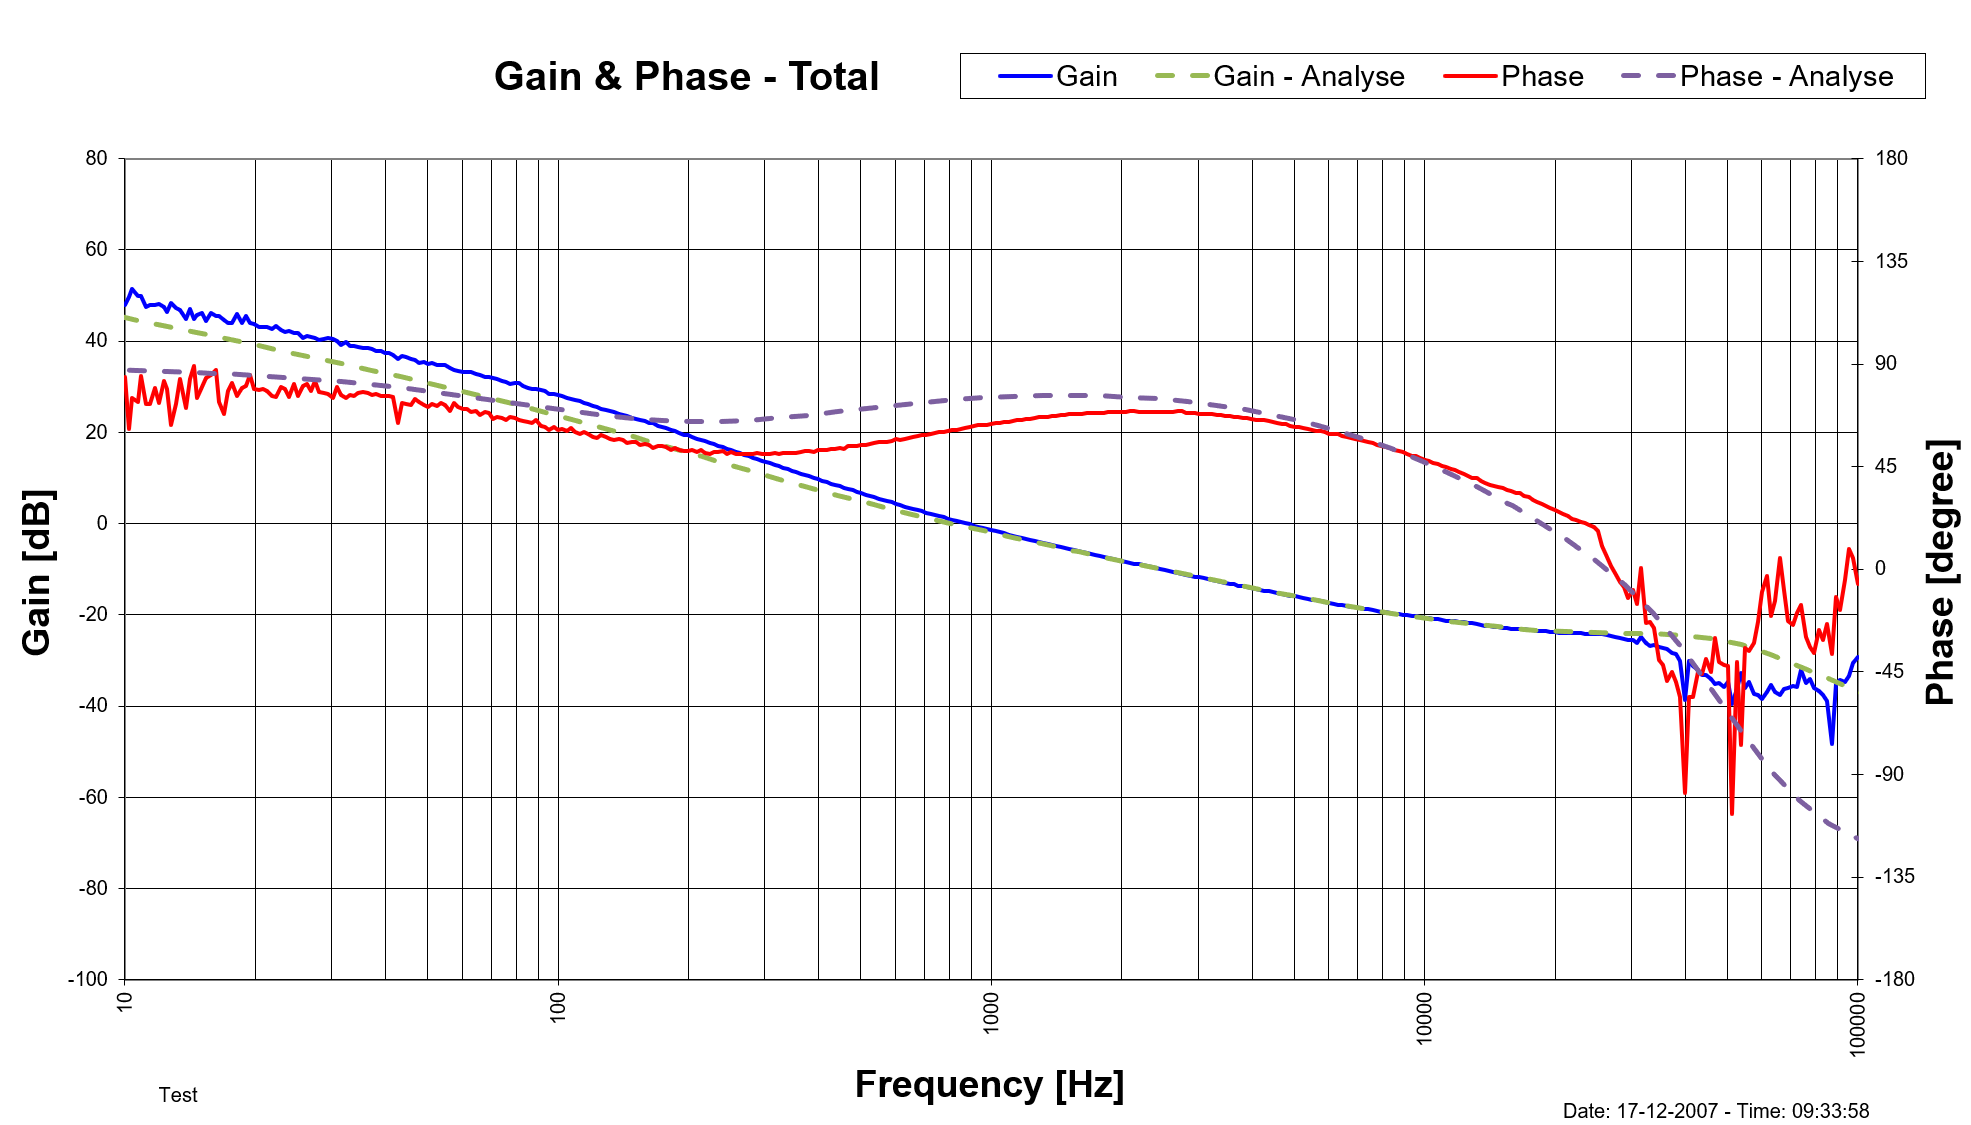
\includegraphics[max width=0.7\linewidth]{../dokumentation/tex/2iteration/billeder/Realisering/Realisering_gain_fase_tot.png}
	\caption{Realiseret og analytisk gain-fase for hele systemet}
	\label{fig:realisering_gain_fase_tot}
\end{figure}
Farverne på linjerne er det samme som ved figur~\ref{fig:realisering_gain_fase_power}. Båndbredden for både analyse og fase aflæses til ca. $900Hz$. For det realiserede aflæses fase-marginen til ca. $62^\circ$ og gain-marginen til ca. $24dB$. Den analyserede fase-margin kan aflæses til $74.3^\circ$ med samme gain-margin som det realiserede.

\subsection{Load step}
Figur~\ref{fig:belastningsamlet} viser det realiserede load step.
\begin{figure}[H]
	\center
	\includegraphics[max width=0.7\linewidth]{../dokumentation/tex/2iteration/billeder/Realisering/belastningsamlet.png}
	\caption{Realisering af load step}
	\label{fig:belastningsamlet}
\end{figure}
Dety aflæses at spændingen falder med ca. 700mV ved overgangen til $10\ohm$. Det tager ca. $1.5ms$ at regulere ind til den stationære værdi. Ved overgangen tilbage til $20\ohm$ stiger spændingen ca. $600mV$, og bruger igen $1.5ms$ på at regulere ind igen.

Tabel~\ref{tab:Loadstep} vises det hvor godt simuleringen og de realiserede målinger stemmer overens.
\begin{table}[H] 			
	\centering
	\begin{tabularx}{\textwidth}{|X|l|l|l|l|}
		\hline
		& \multicolumn{2}{|l|}{\textbf{Simulering}} & \multicolumn{2}{|l|}{\textbf{Realisering}} \\ \hline
		\textbf{Belastning} & $10\ohm$ & $20\ohm$ & $10\ohm$ & $20\ohm$ \\ \hline
		Overshoot & $650mV$ & $700mV$ & $700mV$ & $600mV$  \\ \hline
		Reguleringstid & $1.6ms$ & $1.6ms$ & $1.5ms$ & $1.5ms$ \\ \hline
	\end{tabularx}
	\caption{Simulering og realisering af load step}
	\label{tab:Loadstep}
\end{table}